\section{Introduction}
A single diffusion step can send three distinct image states to the same output. For a coupled family of two-stage steps, we give an exact test for ruling out this loss for every Gaussian posterior denoiser of a compact prior. The two prediction weights must both be nonnegative.

\Cref{fig:collision} illustrates what this test protects. The three source states lie on a line through two images that define an exact posterior denoiser. A coarse Heun step sends all three to the same point. Given the resulting image state, any of the three sources is compatible with the observation, even at zero inversion residual. The log-SNR midpoint DPM-Solver++(2S) step on the same interval sends those sources to three different points. Its output determines which source was used.

The distinction matters when a generative pipeline stores a checkpoint on a trajectory and later needs the preceding state, for instance to replay a stage of an edit. The inverse can know the executed map, endpoints and denoiser and still have only one saved state. Injectivity is the condition for unique recovery under that information contract. A second question is how much work a numerical inverse takes. A third is how closely the forward step follows the intended trajectory.

We study the ordinary discrete step itself. Prior work has solved its residual equation numerically~\cite{hong2024} and shown that an exact one-prediction DDIM step has a unique inverse~\cite{verbii2026}. Here the second prediction consumes a state computed from the first. We show when that coupling admits a global inverse and when it can create multiple roots of the step equation.

\begin{itemize}
\item \textbf{A sharp criterion for two coupled predictions.} Covariance geometry gives a global inverse for nonnegative weights. A fixed two-atom prior gives the converse by making either negative weight dominate at an appropriate input.
\item \textbf{The minimum protected Heun schedule.} The criterion gives a per-step threshold of $1/2$. A collision at the first subthreshold step survives the rest of a fixed schedule, which gives the exact minimum length for universal protection.
\item \textbf{A choice between two successful inverses.} On the separately frozen FFHQ64 panel, both DPM++2S and Heun2 recover all clean sources at the same work ceiling. DPM++2S takes fewer inverse evaluations and Heun2 follows the fine-step trajectory more closely. We measure these properties separately and keep the learned-model comparison distinct from the exact guarantee.
\end{itemize}

\begin{figure*}[t]
\centering
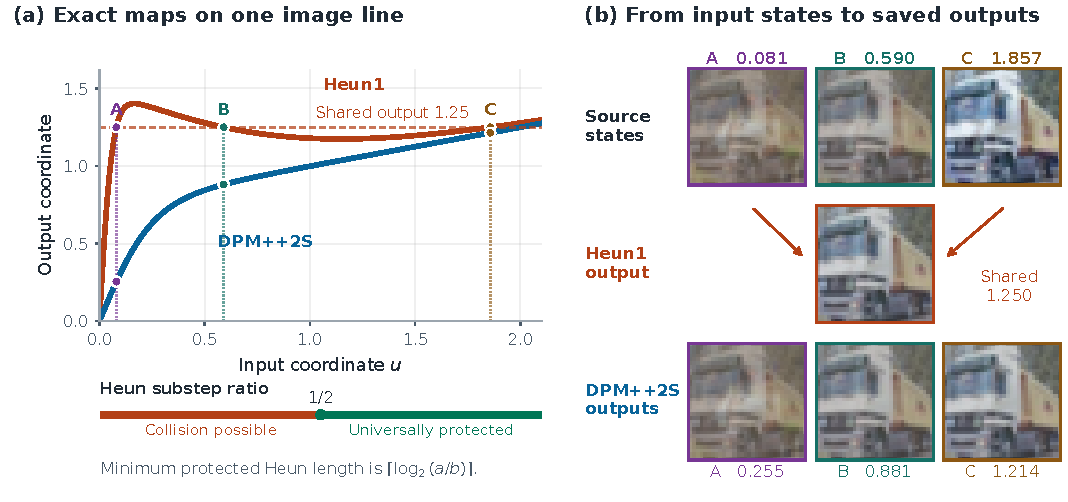
\includegraphics[width=\textwidth]{../figures/figure1.pdf}
\caption{\textbf{One saved Heun output, three compatible inputs.}
\textbf{(a)} The two exact step maps act on the same affine image line $c+uv$ at normalized noise $1\to1/4$. Each of the three marked input brackets contains a root of $H(u)=1.25$, certified by interval arithmetic. DPM++2S separates the same inputs.
\textbf{(b)} The three source tiles are possible reconstructions from the single Heun output. With DPM++2S each source produces a distinct output tile. Below the plot, the ratio rule applies to fixed Heun substeps at positive noise. All tiles use a shared $[-1.8,1.8]$ display mapping because affine states can exceed ordinary image bounds. Displayed coordinates are rounded.}
\label{fig:collision}
\end{figure*}
